%----------------------------------------------------------------------------
\chapter{Hallgatók értékelései}\label{chapter:assessments}
%----------------------------------------------------------------------------

\section{Értékelési rendszer (2-3 oldal)}
A korábban leírtaknak megfelelően a JPorta tárgyaiban lehetőség van különböző értékeléseket felvenni, majd azokat kurzusokhoz rendelni. Ezeket később a kurzus oktatói fogják értékelni.

Új értékelést csak a tárgy adminisztrátorai tudnak létrehozni és kurzusokhoz rendelni. Mindne értékeléshez az alábbi tulajdonságok tartoznak:
\begin{itemize}
    \item Név: rövid név, mely azonosítja az értékelést, pl. ZH 1
    \item Típus: előre definiált értékek, melyekhez tartozik egy reguláris kifejezés \cite{RegExp}. Csak olyan értéket vehet fel, ami illeszkedik a hozzá tartozó kifejezésre.
    \item Súly: meghatározza a sorrendet az értékelések megjelenítésénél.
    \item Ki értékelheti: kurzusokhoz, vagy csak a tárgyhoz rendelt oktatók értékelhetik.
    \item Dinamikus-e: az adott értékelés dinamikusan értékelődik-e ki, ld. \aref{section:dynamic-assessments} pontban.
    \item Privát-e: a privát értékeléseket csak az oktatók látják, a hallgatók nem.
    \item Megjegyzés: részletes leírása az értékelésnek, tipikusan dinamikus értékelések esetén hasznos.
    \item Kurzusok: tárgyon belül mely kurzusokhoz akarjuk hozzárendelni az értékelést.
\end{itemize}

\begin{figure}[h]
    \centering
    \resizebox{\textwidth}{!}{
        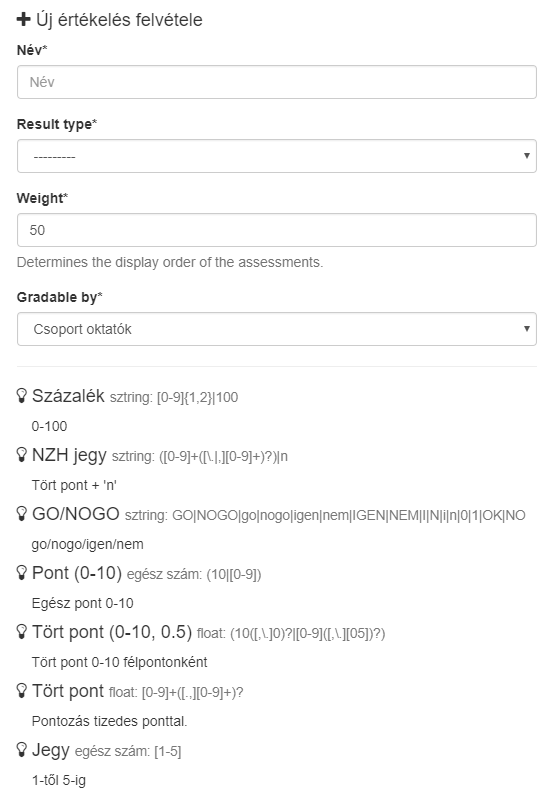
\includegraphics[]{jporta_add_result.png}
    }
    \caption{Értékelés típus hozzáadása}
    \label{fig:jporta_add_result}
\end{figure}

\begin{figure}[h]
    \centering
    \resizebox{\textwidth}{!}{
        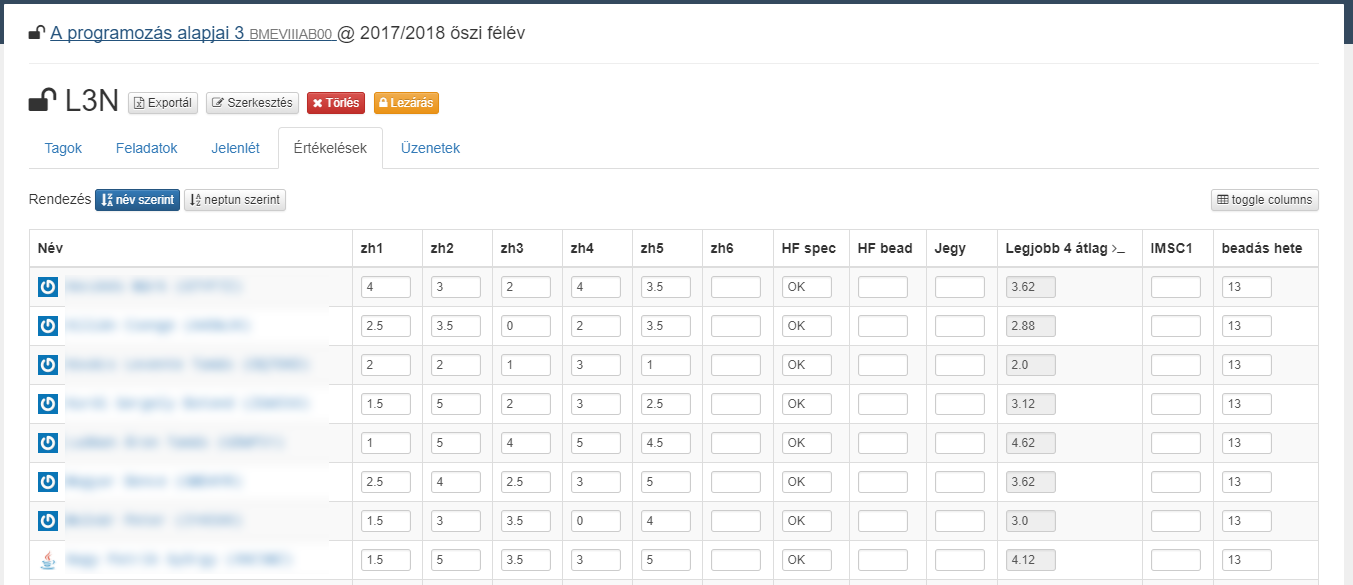
\includegraphics[]{jporta_course_results.png}
    }
    \caption{Hallgatók értékelései}
    \label{fig:jporta_course_results}
\end{figure}

\section{Dinamikus mezők (3-5 oldal)}\label{section:dynamic-assessments}

\subsection{Dinamikus mezők egymásra hivatkozása}